\section{Ergebnisse und Diskussion}
\label{sec:ergebnisseUndDiskussion}
Im nachfolgenden Kapitel werden im ersten Schritt die Ergebnisse der Datenerhebungsmaßnahmen ausgewertet und graphisch aufbereitet. Im zweiten Schritt sollen die aufbereiteten Daten interpretiert, diskutiert und miteinander in Bezug gesetzt werden. Zusätzlich soll eine reduzierte Form der \gls{KNA} durchgeführt werden, um eine Einschätzung über die Wirtschaftlichkeit des Projekts zu erhalten. Als letzten Schritt werden die Hypothesen sowie die Forschungsfrage erneut aufgegriffen und mit Hilfe der gewonnen Erkenntnisse überprüft und beantwortet.  

%%%%%%%%%%%%%%%%%%%%%%%%%%%%%%%%%%%%%%%%%%%%%%%%%%%%%%%%%%%%%%%%%%%%%%%%%%%%

\subsection{Auswertung der Logfiles}
\label{sec:auswertungDerLogfiles}
Die Daten der erhobenen Logfiles befinden sich im Ausgangszustand in einer Oracle Datenbank und können von da aus weiter verarbeitet werden. Um einen ersten Eindruck über die Daten zu bekommen, wurden bereits während der Erhebungen kleinere Datenbankabfragen entwickelt mit denen die Datensätze aggregiert werden konnten. Dadurch konnte frühzeitig sichergestellt werden, dass die Daten ohne Probleme und in zufriedenstellender Form gesammelt und gespeichert werden. Dies sind für die nachfolgenden Auswertungsschritte wichtige Voraussetzungen.

Für genauere Auswertungen wurde die Beobachtung der Daten auf die Ziele der Arbeit fokussiert. Zu Anfang soll sich bewusst erst auf die aufgestellten Kriterien und Metriken bezogen werden. In einem zweiten Schritt sollen dann Auffälligkeiten die währenddessen entdeckt werden weiter verfolgt werden und mögliche Zusammenhänge hinterfragt werden.

\textbf{Bearbeitungszeiten}

\textbf{Maus- und Tastaturanschläge}

\textbf{Weitere Auffälligkeiten und Zusammenhänge}
%%%%%%%%%%%%%%%%%%%%%%%%%%%%%%%%%%%%%%%%%%%%%%%%%%%%%%%%%%%%%%%%%%%%%%%%%%%%

\subsection{Auswertung der Fragebögen}
\label{sec:auswertungDerFrageboegen}
Für die Auswertung der Fragebögen, die im Kapitel \ref{sec:durchfuehrungEvaluation} von den Probanden erhoben wurden, werden alle Datensätze in eine Excel-Tabelle übertragen. Daraufhin werden die Daten so angeordnet, dass jede Zeile einem Bewertungsaspekt aus dem ISO Fragebogen entspricht (siehe Abb. \ref{fig:auswertungsmatrixNeuerDialog} und Anhang \ref{fig:auswertungsmatrixAlterDialog}). Die Ausprägungen für die Bewertung eines Items werden so formatiert, dass sie anstatt von \enquote{$---$} bis \enquote{$+++$} den Werten von -3 (sehr negativ) bis +3 (sehr positiv) entsprechen. Dies hat den Vorteil das anschließend mit den numerischen Werten weiter gerechnet werden kann, da sie ein repräsentatives Abbild der Antworten darstellen und der Ordnung der Likert-Skala entsprechen\footnote{\cite[vgl.][]{Statista}}. Zudem wurden die Kennzahlen in den Auswertungsmatrizen farblich hinterlegt, damit zwischen negativen (rot) und positiven (grün) Bewertungen unterschieden werden kann. Das Rating der 35 Bewertungsaspekte wurde mit Hilfe der Mittelwerte aus den Bewertungen aller Teilnehmer berechnet. Die Benutzerzufriedenheit eines Gestaltungsgrundsatz wird ebenfalls durch den Mittelwert der fünf zuvor berechneten Mittelwerte der Bewertungsaspekte gebildet und besitzt anschließend einen Wert zwischen -3 und +3. Aus Darstellungsgründen wurden die Zahlen im Folgenden alle auf drei Stellen nach dem Komma gerundet.

In Abbildung \ref{fig:auswertungsmatrixNeuerDialog} sind alle Einschätzungen zu dem neuen Vermögensverzeichnis Dialog in aggregierter Form dargestellt. Stellt man diese Auswertungsmatrix in einen direkten Vergleich zu den Auswertungen des alten Dialogs (siehe Abb. \ref{fig:auswertungsmatrixAlterDialog}) lässt sich erkennen, dass der neue Dialog in allen sieben Gestaltungsgrundsätzen besser bewertet wurde, als der alte Dialog (siehe Abb. \ref{fig:vergleichBalkendiagramm}). 
\begin{figure}[H]
  \centering
  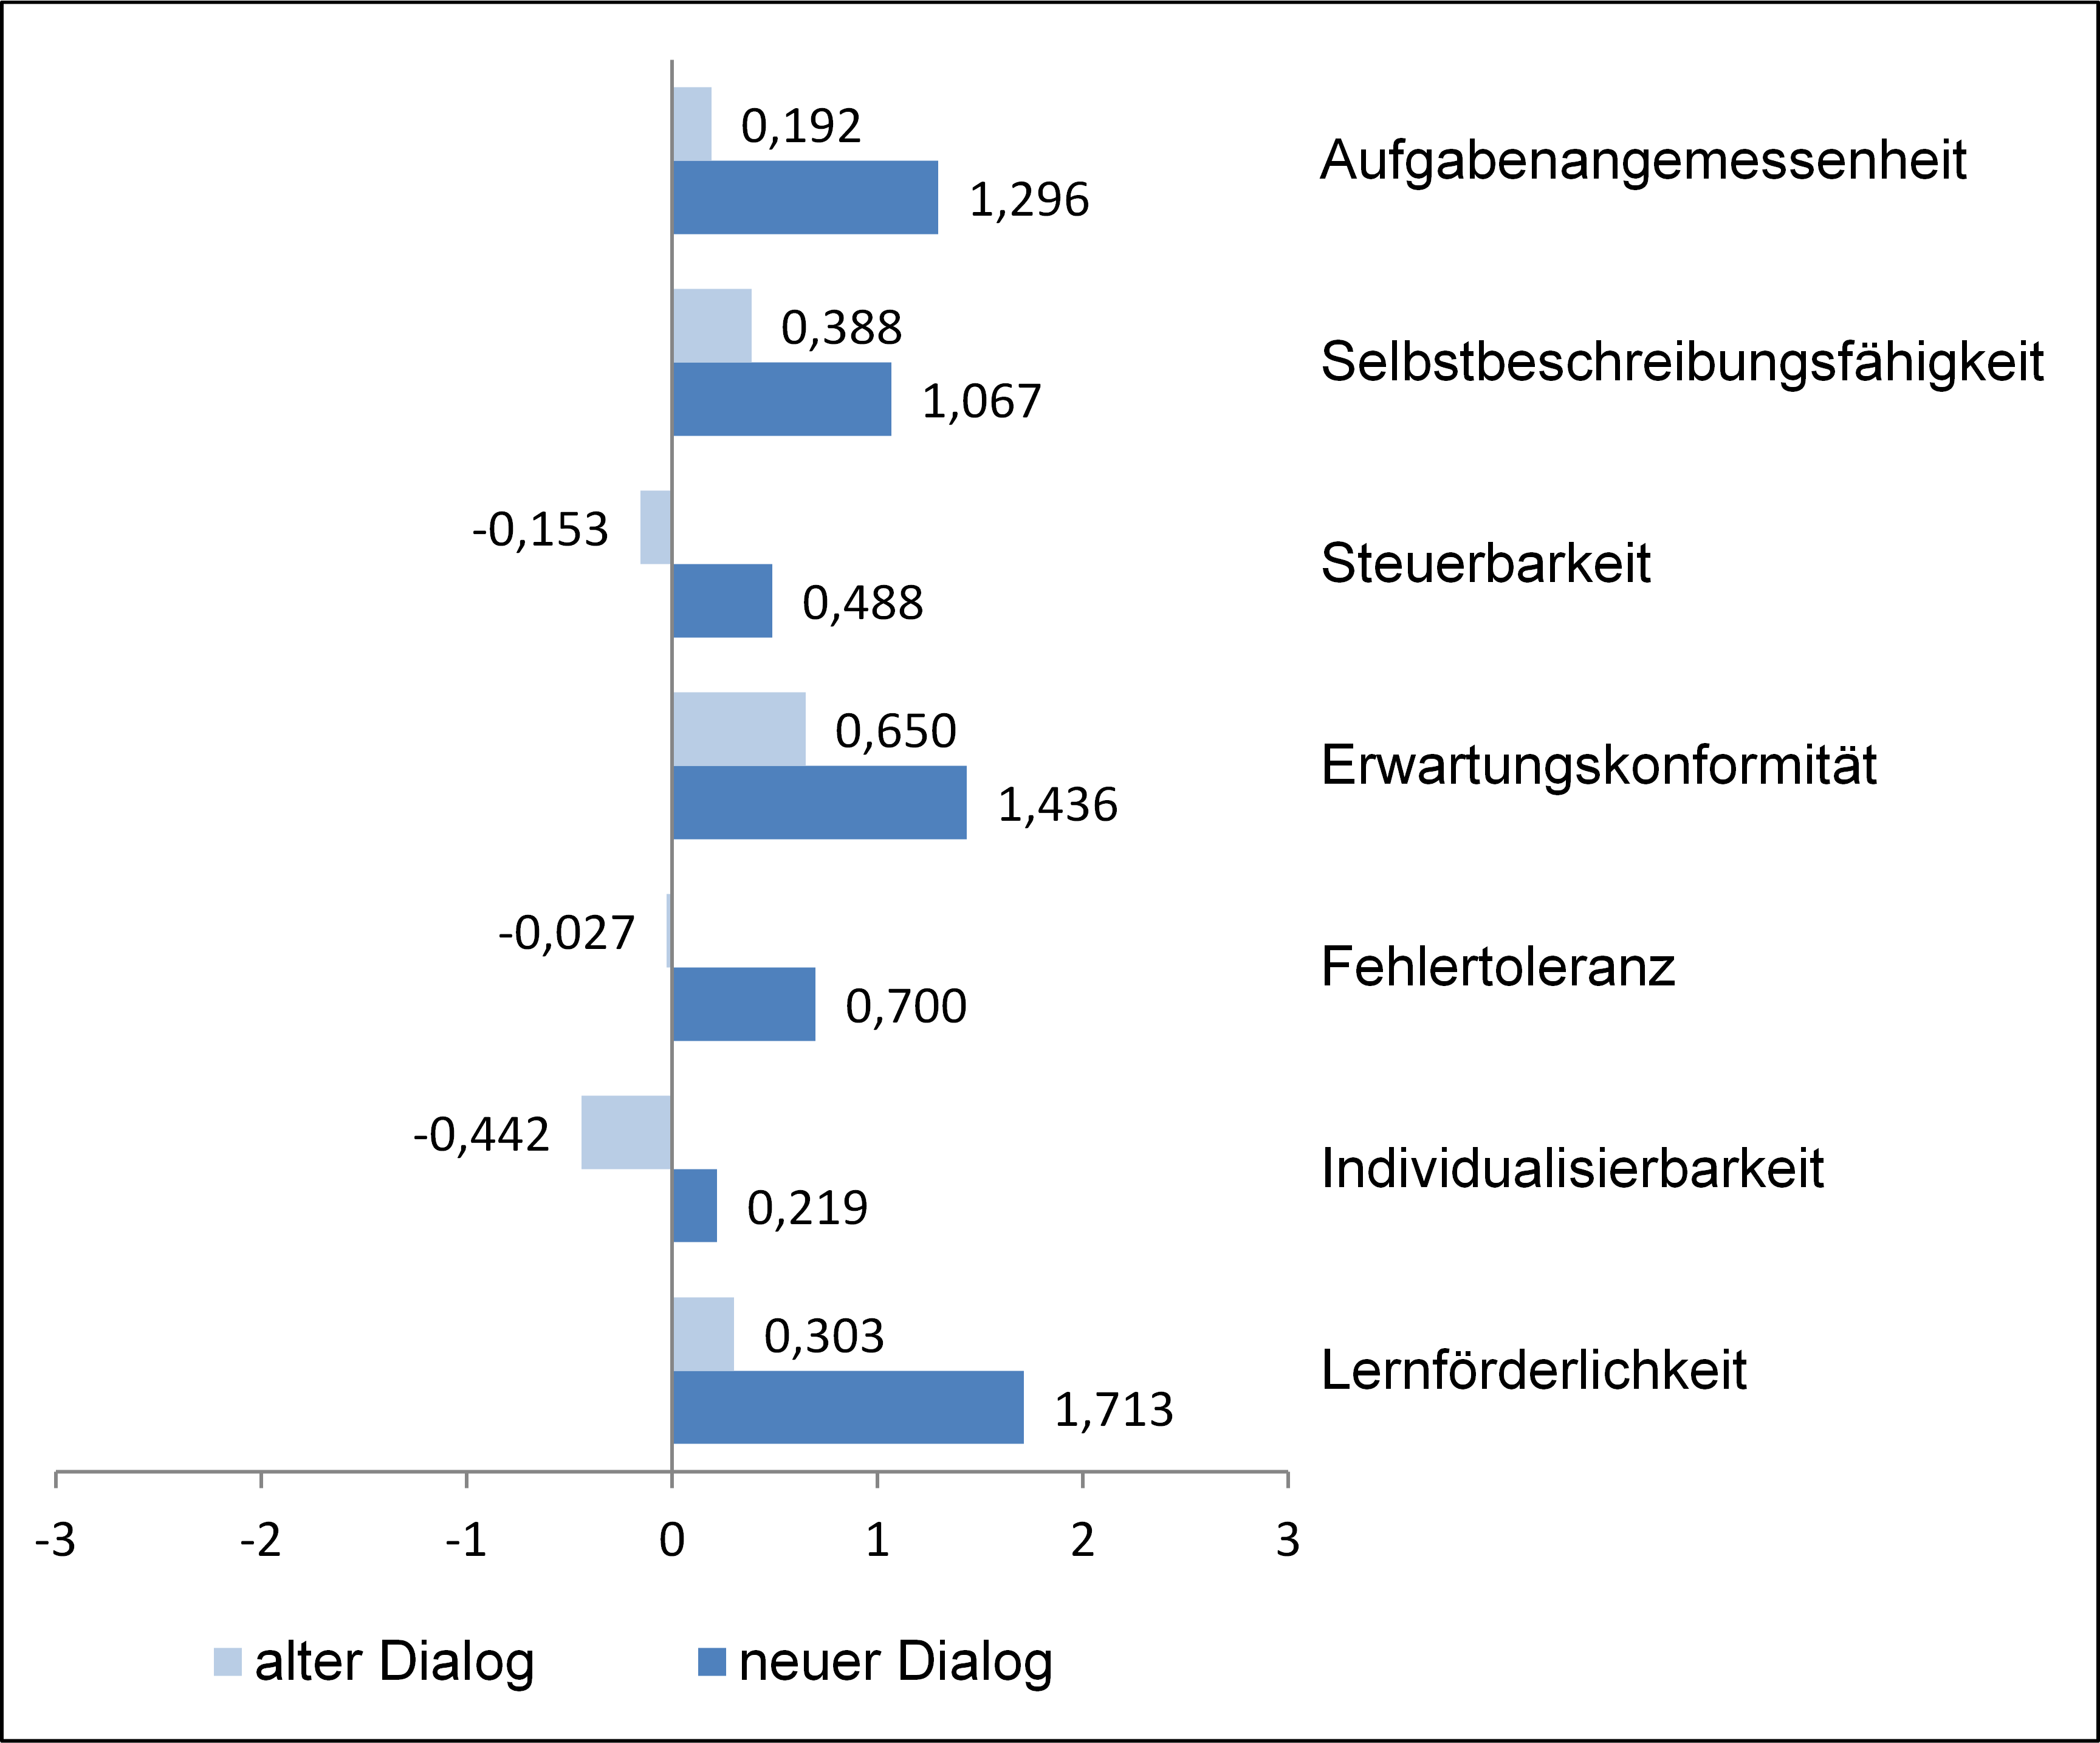
\includegraphics[]{img/ISO9241-10_Vergleich_Balkendiagramm.PNG}
  \caption{Vergleich der Gestaltungsgrundsätze zwischen altem und neuen Dialog.}
  \caption*{\textbf{Quelle:} Eigene Darstellung}
  \label{fig:vergleichBalkendiagramm}
\end{figure}
Die größte Steigerung kann in den Gebieten Aufgabenangemessenheit und Lernförderlichkeit mit 1,1 Punkten und 1,4 Punkten verzeichnet werden. Am wenigsten konnte die Benutzerzufriedenheit bei der Steuerbarkeit und der Individualisierbarkeit steigen. 

Trotz der insgesamt positiven Ergebnisse, gibt es immer noch Bereiche in denen die Bewertungen eher schwach ausfallen. Dazu zählt auch die Steuerbarkeit des Dialogs. Diese ist zwar positiv, also bietet ausreichend Freiheit bei der Bedienung, jedoch empfinden die Benutzer die Unterbrechungsfreiheit und die Anpassbarkeit von Informationsdarstellungen noch nicht vollkommen zufriedenstellend. Dieses Thema ist eher komplex zu bewerten, da hier auf die einzelnen Wünsche und Belangen der einzelnen Sachbearbeiter eingegangen werden müsste, um weitere Verbesserungen zu erzielen.

Auch die Kategorie Individualisierbarkeit selbst konnte im direkten Vergleich einen Gewinn von knapp 0,7 Punkte verzeichnen. Jedoch liegt die Bewertung mit +0,219 im unteren positiven Bereich. Besonders die Punkte \enquote{Erweiterbarkeit durch den Benutzer} und \enquote{Individuelle Anpassbarkeit durch den Benutzer} fallen beide noch schlecht aus. Gleichzeitig sind die beiden Bewertungsaspekte, trotz ihres Anstiegs um 0,4 bzw. 0,6 Punkten, auch die einzigen die noch negativ bewertet wurden. Sie spiegeln die individuelle Erweiterbarkeit und Anpassbarkeit von Bearbeitungsschritte und Benutzer wider. Die Kritik an dieser Stelle ist aber durchaus nachzuvollziehen, da sich der Dialog nur an wenigen Stellen individuell anpassen lässt. Ein Grund dafür ist die niedrige Priorisierung von individuellen und dynamischen Strukturen während der Konzeptionsphase. Es ist denkbar in einem nachfolgenden Projekt noch einmal explizit auf die beiden Aspekte und Benutzeranliegen einzugehen, um bestenfalls die Benutzerzufriedenheit weiter zu verbessern.

Insgesamt ist die Selbstbeschreibungsfähigkeit mit einem Wert von +1,067 durchaus zufriedenstellend. In Bezug auf die, durch den Benutzer geforderten und die durch das System automatisierten Erklärungen, ist aber noch klar ein Verbesserungspotential zu erkennen. Hier könnten gezielte Maßnahmen eingeleitet werden, bei denen zusammen mit dem Fachbereich fehlende Erklärungen evaluiert und anschließend ergänzt werden. Dies sollte einen vergleichsweise geringen Aufwand darstellen und kann auf der anderen Seite große Effekte erzielen.

Mit dem Blick auf die positiven Eigenschaften des neuen Vermögensverzeichnis Dialogs fallen unter die besten fünf Punkte:
\begin{enumerate}
    \item Hilfe beim Behalten von Gelerntem (+2,104),
    \item Autodidaktisch\footnote{Autodidaktisch = Wissen durch Literatur, Übungen, Beobachtungen oder Versuche eigenständig aneignen } (+2,085),
    \item Bedienungskomplexität (+2,083),
    \item Zeit für Einarbeitung (+2,063) und
    \item Erfordernis, sich Details zu merken (+1,979).
\end{enumerate}
Interessant ist, dass vier der fünf Punkte aus dem Bereich Lernförderlichkeit stammen. Der Aspekt \enquote{Bedienungskomplexität} wiederum gehört zum Grundsatz Aufgabenangemessenheit. Hier bewerten die Benutzer die Bedienung des neuen Dialogs, mit einem durchschnittlichen Schwellwert von etwa +2, als angenehm und einfach. Im Vergleich ist dies ein Anstieg von über 1,6 Punkten. Die gestiegene Benutzerzufriedenheit von über 1,4 Punkten im Bereich der Lernförderlichkeit kann genauso wie die Bedienungskomplexität durch die Vereinfachung und Verringerung von Informationen, Bedienelementen und Strukturen erklärt werden. 
\begin{figure}[H]
  \centering
  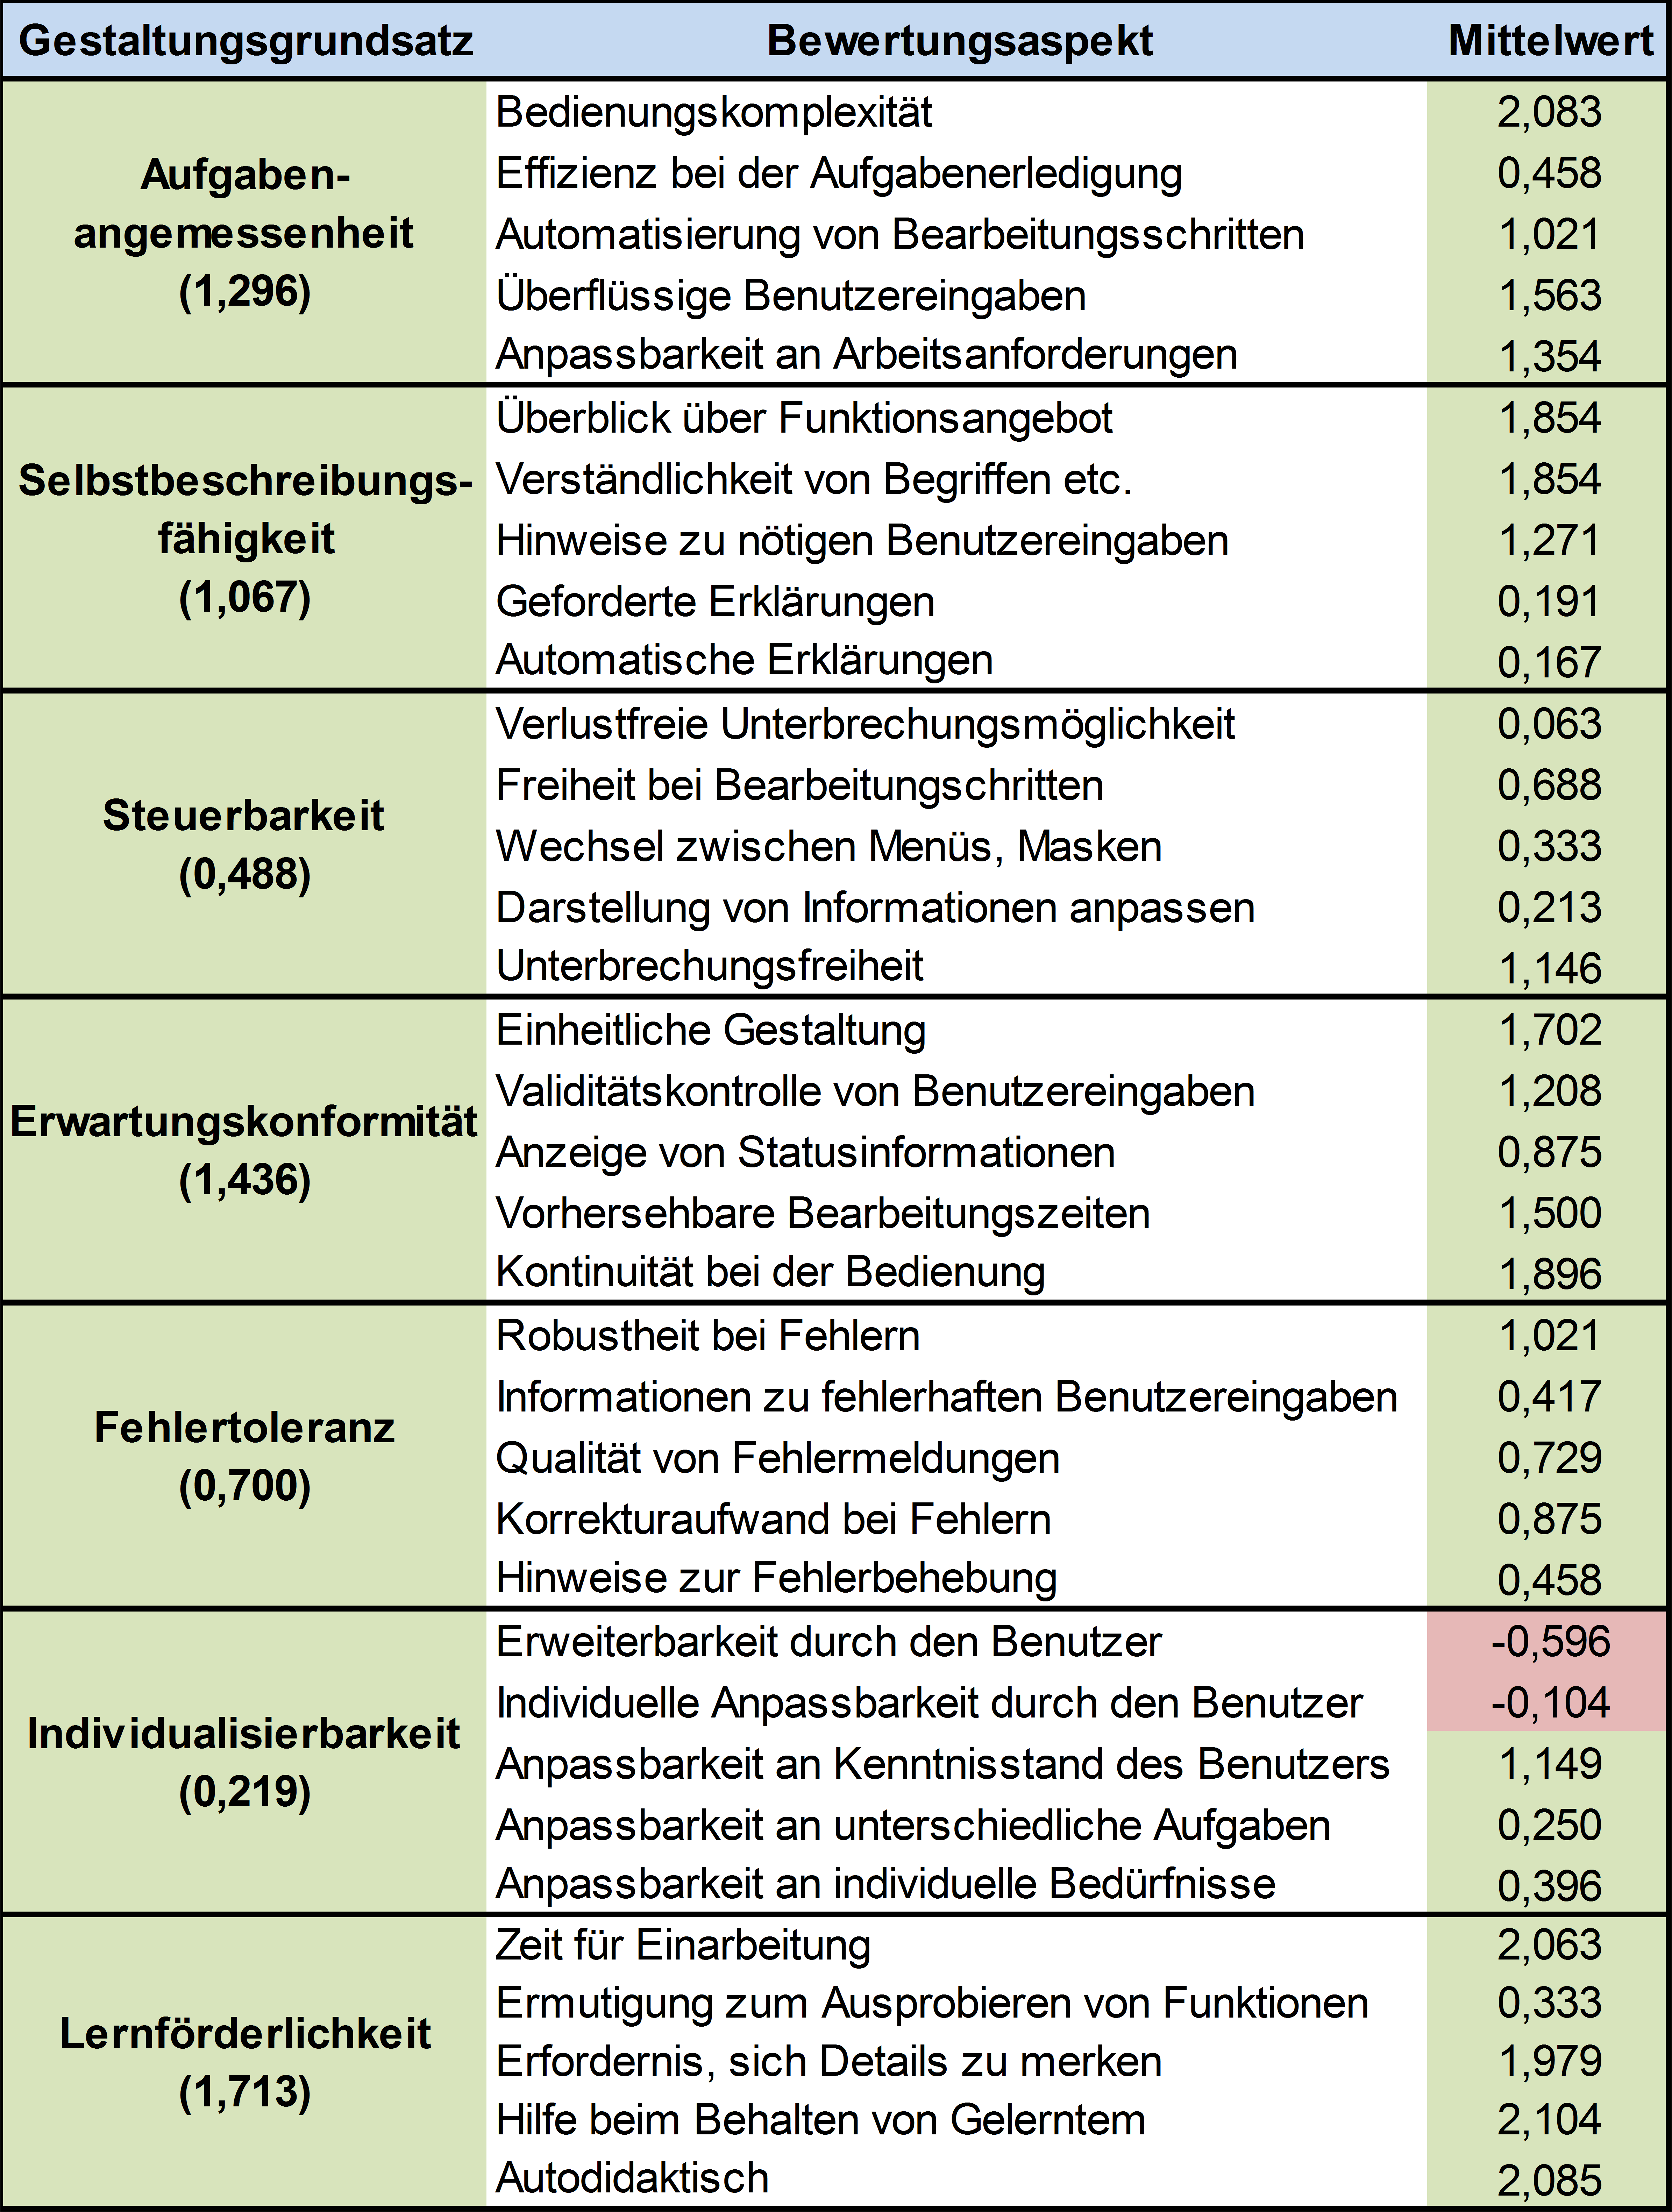
\includegraphics[width=430px]{img/Auswertungsmatrix_Neuer_Dialog.PNG}
  \caption{Auswertungsmatrix zum ISO 9241-10 Fragebogen neuer Dialog.}
  \caption*{\textbf{Quelle:} Eigene Darstellung}
  \label{fig:auswertungsmatrixNeuerDialog}
\end{figure}
Die fünf Bewertungsaspekte sollten gerade mit Blick auf die Zeit positive Auswirkungen haben. Fällt die Betrachtung auf die Punkte zwei und vier so lässt sich ableiten, dass potentiell künftig Zeit eingespart werden kann. Es muss sich lediglich der Anwendungsfall \enquote{Neuer Mitarbeiter} vorgestellt werden. Der neue Mitarbeiter benötigt tendenziell weniger Zeit für die Einarbeitung in den neuen Dialog. Zudem kann der zeitliche Aufwand für helfende und einweisende Kollegen verringert werden.

So lassen sich auch die Punkte \enquote{Erfordernis, sich Details zu merken} und \enquote{Hilfe beim Behalten von Gelerntem} mit einer gesteigerten Effizienz in Verbindung bringen. Ein möglicher Anwendungsfall hierfür ist ein Vermögensverzeichnis, das viele Details enthält. Hier muss der Sachbearbeiter im Gegensatz zum alten Dialog nur noch einen Bruchteil der Informationen übernehmen und somit auch weniger Informationen gleichzeitig im Gedächtnis behalten. Dies kann durchaus positive Effekte auf die Bearbeitungszeit und die mentale Belastung des Sachbearbeiters nehmen.

Im Gesamtüberblick kann bereits ein erfreulicher Verlauf der Benutzerzufriedenheit in allen sieben Grundsätzen verzeichnet werden. Hieraus lässt sich bereits auf eine gewisse Effektivität des Projekts schließen, besonders mit Bezug auf die zeitlichen Effekte. Die Benutzer scheinen allgemein zufriedener bei der Arbeit mit dem neuen Dialog.

%%%%%%%%%%%%%%%%%%%%%%%%%%%%%%%%%%%%%%%%%%%%%%%%%%%%%%%%%%%%%%%%%%%%%%%%%%%%

\subsection{Bewertung der Wirtschaftlichkeit}
\label{sec:KNAZusaetzlichesKriterium}

%%%%%%%%%%%%%%%%%%%%%%%%%%%%%%%%%%%%%%%%%%%%%%%%%%%%%%%%%%%%%%%%%%%%%%%%%%%%

\subsection{Zusammenfassung}
\label{sec:zusammenfassung}